\documentclass[11pt, oneside]{article}   	% use "amsart" instead of "article" for AMSLaTeX format
\usepackage{geometry}                		% See geometry.pdf to learn the layout options. There are lots.
\geometry{letterpaper}                   		% ... or a4paper or a5paper or ... 
%\geometry{landscape}                		% Activate for for rotated page geometry
%\usepackage[parfill]{parskip}    		% Activate to begin paragraphs with an empty line rather than an indent
\usepackage{graphicx}				% Use pdf, png, jpg, or eps� with pdflatex; use eps in DVI mode
								% TeX will automatically convert eps --> pdf in pdflatex		
\usepackage{amssymb}
\graphicspath{{/Users/telliott_admin/Dropbox/Tex/png/}}
\usepackage{parskip}

\title{Surface Area and Volume}
\date{}
\begin{document}
\maketitle
\Large

\subsection*{Volumes}

One of the great things about calculus is the discovery that one can use integration to compute surface areas and volumes.  

Let's start with a simple example:  a (right circular) cone, one whose cross-section at each height is a circle, and whose vertex lies directly on the altitude, which runs through the center of all the circles.

To make it even simpler, to begin with we will have the radius of the base $R$ be equal to the height $H$, so at each height $h$, $r=h$.

Lay the cone on its side with the vertex at the origin and the altitude coinciding with the $x$-axis, except let's rename it as the $h$-axis.  Imagine slicing perpendicular to the $h$-axis.  We add up all the slices from $h=0 \rightarrow h=H$.  For each slice, the area of the slice is 
\[ A(h) = \pi r^2 \]
but $r=h$ so
\[ A(h) = \pi h^2 \]

We sum them all up by doing 
\[ \int A(h) \ dh = \int_0^H \pi h^2 \ dh \]
\[ V = \frac{1}{3} \pi h^3 \ \bigg |_0^H =  \frac{1}{3} \pi H^3 \]

Now, let's modify the problem to use a cone with a different ratio of $R/H$.  We have this relationship between the radius $r$ of each cross-section and the height $h$ at that point

\[ \frac{r}{h} = \frac{R}{H} \]
so
\[ r = \frac{R}{H} h \]
As before
\[ A(h) = \pi r^2 \]
But now
\[ A(h) = \pi \frac{R^2}{H^2} h^2 \]

We sum them all up by doing 
\[ \int A(h) \ dh \]
\[ = \int_0^H \pi \frac{R^2}{H^2} h^2 \ dh \]
\[ = \frac{R^2}{H^2} \int_0^H \pi h^2 \ dh \]
So all we do is to modify our previous answer by multiplying
\[ V =  \frac{R^2}{H^2} \times \frac{1}{3} \pi H^3 \]
\[ = \frac{1}{3} \pi R^2 H \]

This method is called the method of "disks".  We can do much more with this, but I will continue that in the write-up called "Cone and Sphere."

\subsection*{Surface Area}

Let's take a look at surface area.

Suppose we revolve a function $y = f(x)$ around the x-axis.  We imagine slicing it into disks in the usual way, moving along the $x$-axis in increments $dx$.  To compute the surface area of the solid, we might try adding up the perimeter of all the disks.
Suppose we try the simple cone with $R=H$.  What we have is the function
\[ r = h \]
The circumference at any point $h$ is
\[ C(h) = 2 \pi r \]
\[ = 2 \pi h \]
And the surface area is
\[ SA = \int C(h) \ dh \]
(this has a subtle error that we will fix).
\[ = \int_0^H 2 \pi h \ dh \]
\[ = \pi h^2  \ \bigg |_0^H \]
\[ =  \pi H^2 = \pi R^2  \]

Now, this is obviously not the correct answer.

We can look it up, or we can try to calculate it directly.  Imagine cutting the surface of our cone directly up along the slant and then opening it and laying it flat.  What we will end up with is a part (sector) of a circle.  

\begin{center} 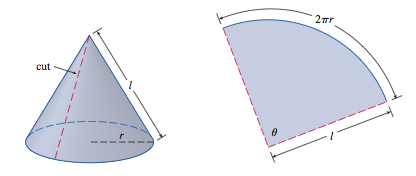
\includegraphics [scale=0.5] {cut_cone.png} \end{center}

The radius of that circle is the slant height of the cone.

\[ S = \sqrt{R^2 + H^2} \]
Its total circumference would be $2 \pi S$.

However, the arc length along the sector that we actually have is the circumference of the base of the cone, which is just $2 \pi R$.

So the total area of the sector (equivalent to the surface area of the cone) is the total area of the circle, times the ratio of the sector circumference to the total circumference.

\[ SA = \pi S^2 \ \frac{2 \pi R}{2 \pi S} = \pi RS \]

The error in our application of calculus to this problem is a factor of $S/R$.

It turns out that what we did wrong is to multiply the circumference at each point by $dx$.  What we should have done is to multiply it by the little increment of slant instead.

Since 
\[ S = \sqrt{R^2 + H^2} \]

and in this problem
\[ R = H \]
\[ S = \sqrt{2} R \]

So the answer we obtained was $\pi R^2$, whereas the correct answer is $\pi R S$, and in this problem $S =  \sqrt{2} R$, so that's just $\sqrt{2} \pi R^2$.

\subsection*{General approach}

Let me return to our more traditional notation of $x$ and $y$.  We have some function $y=f(x)$ and we think of rotating this function around the $x$-axis.  The length that we need to multiply with is not $dx$ or $dy$ but the hypotenuse of the triangle that they form together, namely

\[ ds^2 = dx^2 + dy^2 \]
\[ ds^2 = (1 + \frac{dy}{dx})^2 \ dx^2 \]
\[ ds = \sqrt{1 + (\frac{dy}{dx})^2} \ dx \]
\[ ds = \sqrt{1 + f'(x)^2} \ dx \]
After setting up ds, we will integrate
\[ \int 2 \pi y \ ds \]
\[ \int 2 \pi y \ \sqrt{1 + f'(x)^2} \ dx \]

Returning  to the general cone problem, we have 
\[ y = \frac{R}{H} x \]
\[ f'(x) = \frac{R}{H} \]
\[ ds = \sqrt{1 + \frac{R^2}{H^2}} \ dx \]

So our integral is
\[ \int 2 \pi y \ \sqrt{1 + f'(x)^2} \ dx \]
\[ = \int_0^H 2 \ \pi \frac{R}{H} x \ \sqrt{1 + \frac{R^2}{H^2}} \ dx \]
\[ = \pi \frac{R}{H} \ \sqrt{1 + \frac{R^2}{H^2}} \int_0^H 2 x \ dx \]
\[ = \pi \frac{R}{H} \ \sqrt{1 + \frac{R^2}{H^2}} \ (H^2)  \]
\[ = \pi RH \ \sqrt{1 + \frac{R^2}{H^2}}  \]
We can also clean up the result above by bringing the $H$ inside the square root

\[ = \pi R \ \sqrt{H^2 + R^2}  \]
This is $\pi R S$.  In our particular example of the right circular cone, $R=H$ so we have just
\[ SA = \sqrt{2} \pi R^2 \]

\subsection*{Last example}

Consider the circle with radius R centered at the origin.
\[ 
x^2 + y^2 = R^2 \]
\[ y = f(x) = \sqrt{R^2 - x^2}
\]
Using implicit differentiation, it is easy to show that
\[  2x \ dx + 2y \ dy = 0 \]
\[  \frac{dy}{dx} = -x/y \]
Then
\[ ds = \sqrt{1 + \frac{x^2}{y^2}} \ dx \]
\[ =  \sqrt{1 + \frac{x^2}{(R^2 - x^2)}} \ dx \]
And
\[ S = 2 \pi \int y \ ds \]
\[ = 2 \pi \int   \sqrt{(R^2-x^2)} \  \sqrt{1 + \frac{x^2}{(R^2 - x^2)}} \ dx \]
\[ = 2 \pi \int   \sqrt{R^2 - x^2 + x^2 } \ dx \]
\[ = 2 \pi \int R \  dx \]
\[ = 2 \pi R x \]
evaluate from $x = -R \rightarrow R$, giving:
\[ S = 4 \pi R^2 \]
The expected result.

\end{document}  